%Notes by Harsh Mistry 
%CS 349
%Based on Template From  https://www.cs.cmu.edu/~ggordon/10725-F12/template.tex

\documentclass[twoside]{article}
\setlength{\oddsidemargin}{0.25 in}
\setlength{\evensidemargin}{-0.25 in}
\setlength{\topmargin}{-0.6 in}
\setlength{\textwidth}{6.5 in}
\setlength{\textheight}{8.5 in}
\setlength{\headsep}{0.75 in}
\setlength{\parindent}{0 in}
\setlength{\parskip}{0.1 in}
\usepackage{amsmath,amsfonts,graphicx}
\newcounter{lecnum}
\renewcommand{\thepage}{\thelecnum-\arabic{page}}
\renewcommand{\thesection}{\thelecnum.\arabic{section}}
\renewcommand{\theequation}{\thelecnum.\arabic{equation}}
\renewcommand{\thefigure}{\thelecnum.\arabic{figure}}
\renewcommand{\thetable}{\thelecnum.\arabic{table}}
\newcommand{\lecture}[4]{
   \pagestyle{myheadings}
   \thispagestyle{plain}
   \newpage
   \setcounter{lecnum}{#1}
   \setcounter{page}{1}
   
   
%Info Box 
   \begin{center}
   \framebox{
      \vbox{\vspace{2mm}
    \hbox to 6.28in { {\bf CS 349 - User Interfaces
	\hfill Winter 2018} }
       \vspace{4mm}
       \hbox to 6.28in { {\Large \hfill Lecture #1: #2  \hfill} }
       \vspace{2mm}
       \hbox to 6.28in { {\it Lecturer: #3 \hfill Notes By: #4} }
      \vspace{2mm}}
   }
   \end{center}
   
   \markboth{Lecture #1: #2}{Lecture #1: #2}



 
}

\renewcommand{\cite}[1]{[#1]}
\def\beginrefs{\begin{list}%
        {[\arabic{equation}]}{\usecounter{equation}
         \setlength{\leftmargin}{2.0truecm}\setlength{\labelsep}{0.4truecm}%
         \setlength{\labelwidth}{1.6truecm}}}
\def\endrefs{\end{list}}
\def\bibentry#1{\item[\hbox{[#1]}]}

\newcommand{\fig}[3]{
			\vspace{#2}
			\begin{center}
			Figure \thelecnum.#1:~#3
			\end{center}
	}
	
\graphicspath{ {images/} }

\newtheorem{theorem}{Theorem}[lecnum]
\newtheorem{lemma}[theorem]{Lemma}
\newtheorem{ex}[theorem]{Example}
\newtheorem{proposition}[theorem]{Proposition}
\newtheorem{claim}[theorem]{Claim}
\newtheorem{corollary}[theorem]{Corollary}
\newtheorem{definition}[theorem]{Definition}
\newenvironment{proof}{{\bf Proof:}}{\hfill\rule{2mm}{2mm}}
\newcommand\E{\mathbb{E}}


%Start of Document 
\begin{document}

\lecture{7}{January 18, 2018}{Keiko Katsuragawa}{Harsh Mistry}

\section{Event Dispatch}

\subsection{Event Architecture}

\begin{itemize}
\item A pipeline 
\begin{itemize}
\item Capture and Queue low-level hardware events
\item Dispatch events correct window and widget 
\item Bind event with application code
\end{itemize}
\end{itemize}

\begin{center}
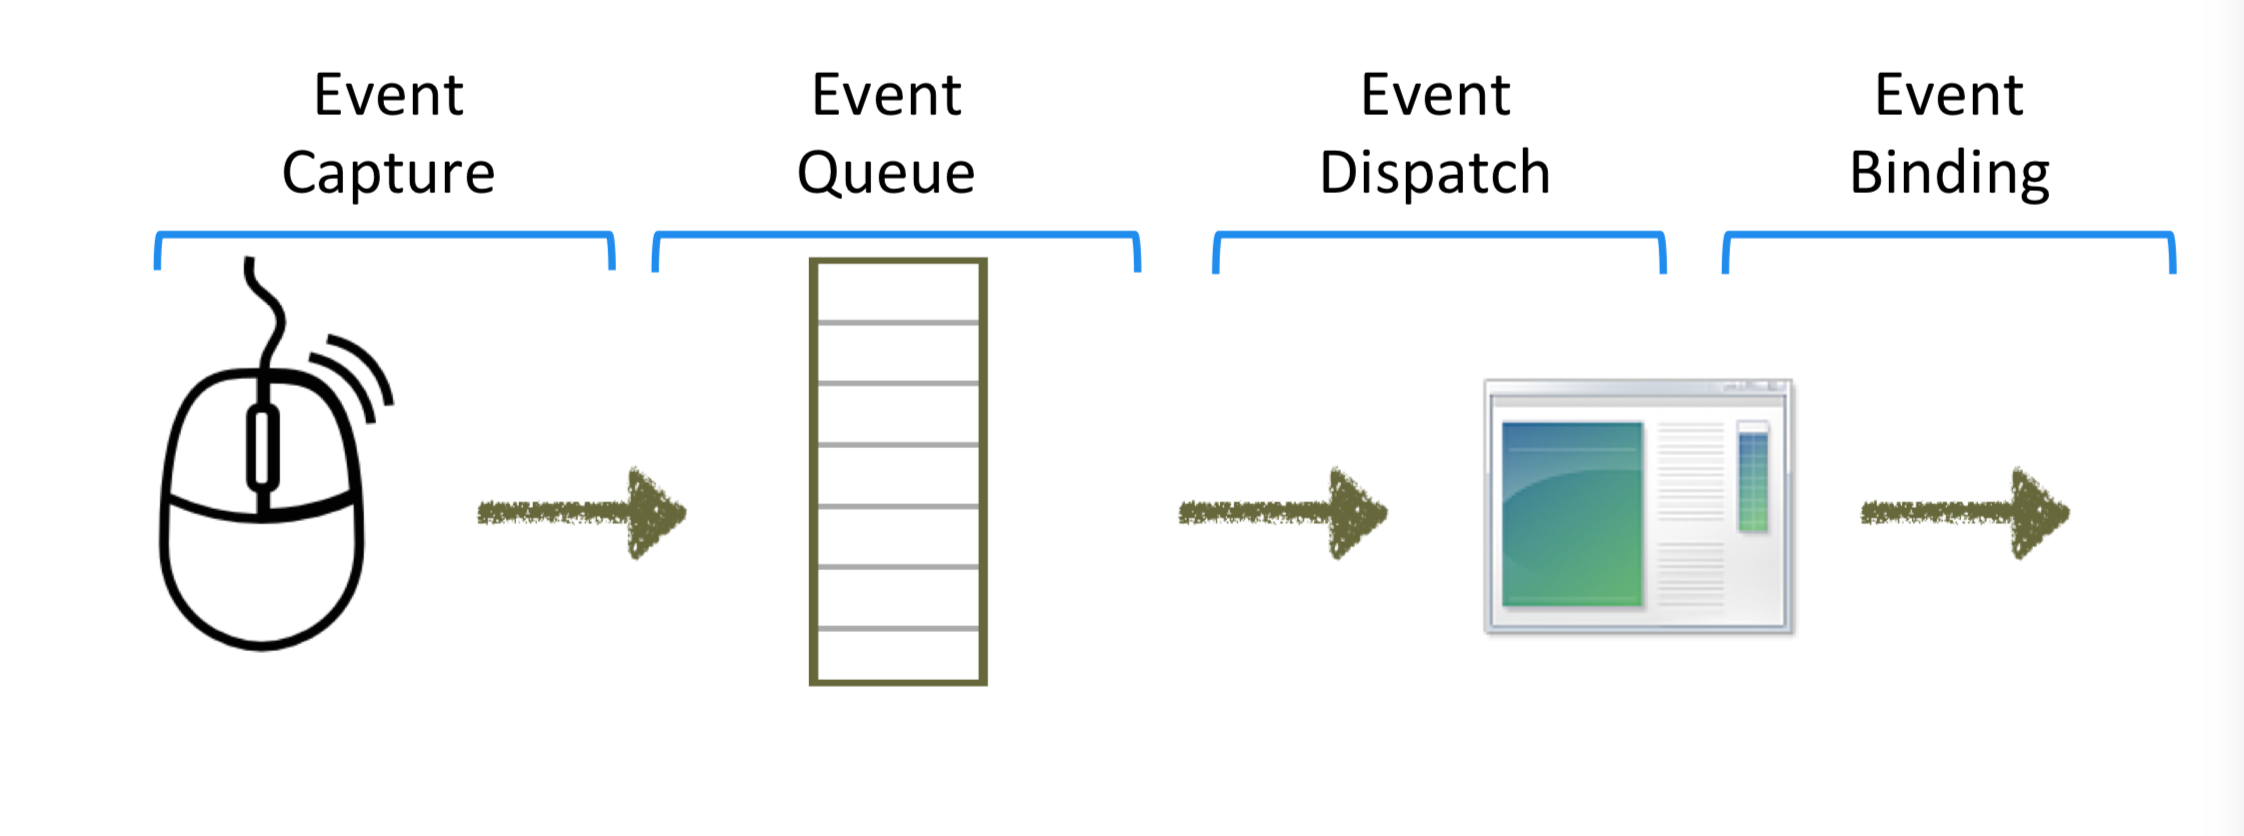
\includegraphics[scale=0.3]{24}
\end{center}

\subsection{Event Loop}
\begin{itemize}
\item Iterate through event queue, and dispatch event to handler(s) -  Low-level mechanism for event dispatch
\item BWS event queue always dispatches to an application window 
\begin{itemize}
\item what window triggered the event
\item what window has mouse or keyboard “focus”
\end{itemize}
\item Final dispatch depends on what manages application-level events: 
\begin{itemize}
\item BWS could dispatch to widget level (heavyweight)
\item application could manage dispatch (lightweight, e.g. Xlib)
\item toolkit could dispatch to widgets (lightweight, JVM/Swing)
\end{itemize}

\end{itemize}

\subsection{Interactor Tree}
\begin{itemize}
\item 2D layout of widgets forms a hierarchy 
\item COntainer widgets are ancestors of simple widgets 
\item Dispatching an event is done by traversing the interactor tree 
\end{itemize}

\begin{center}
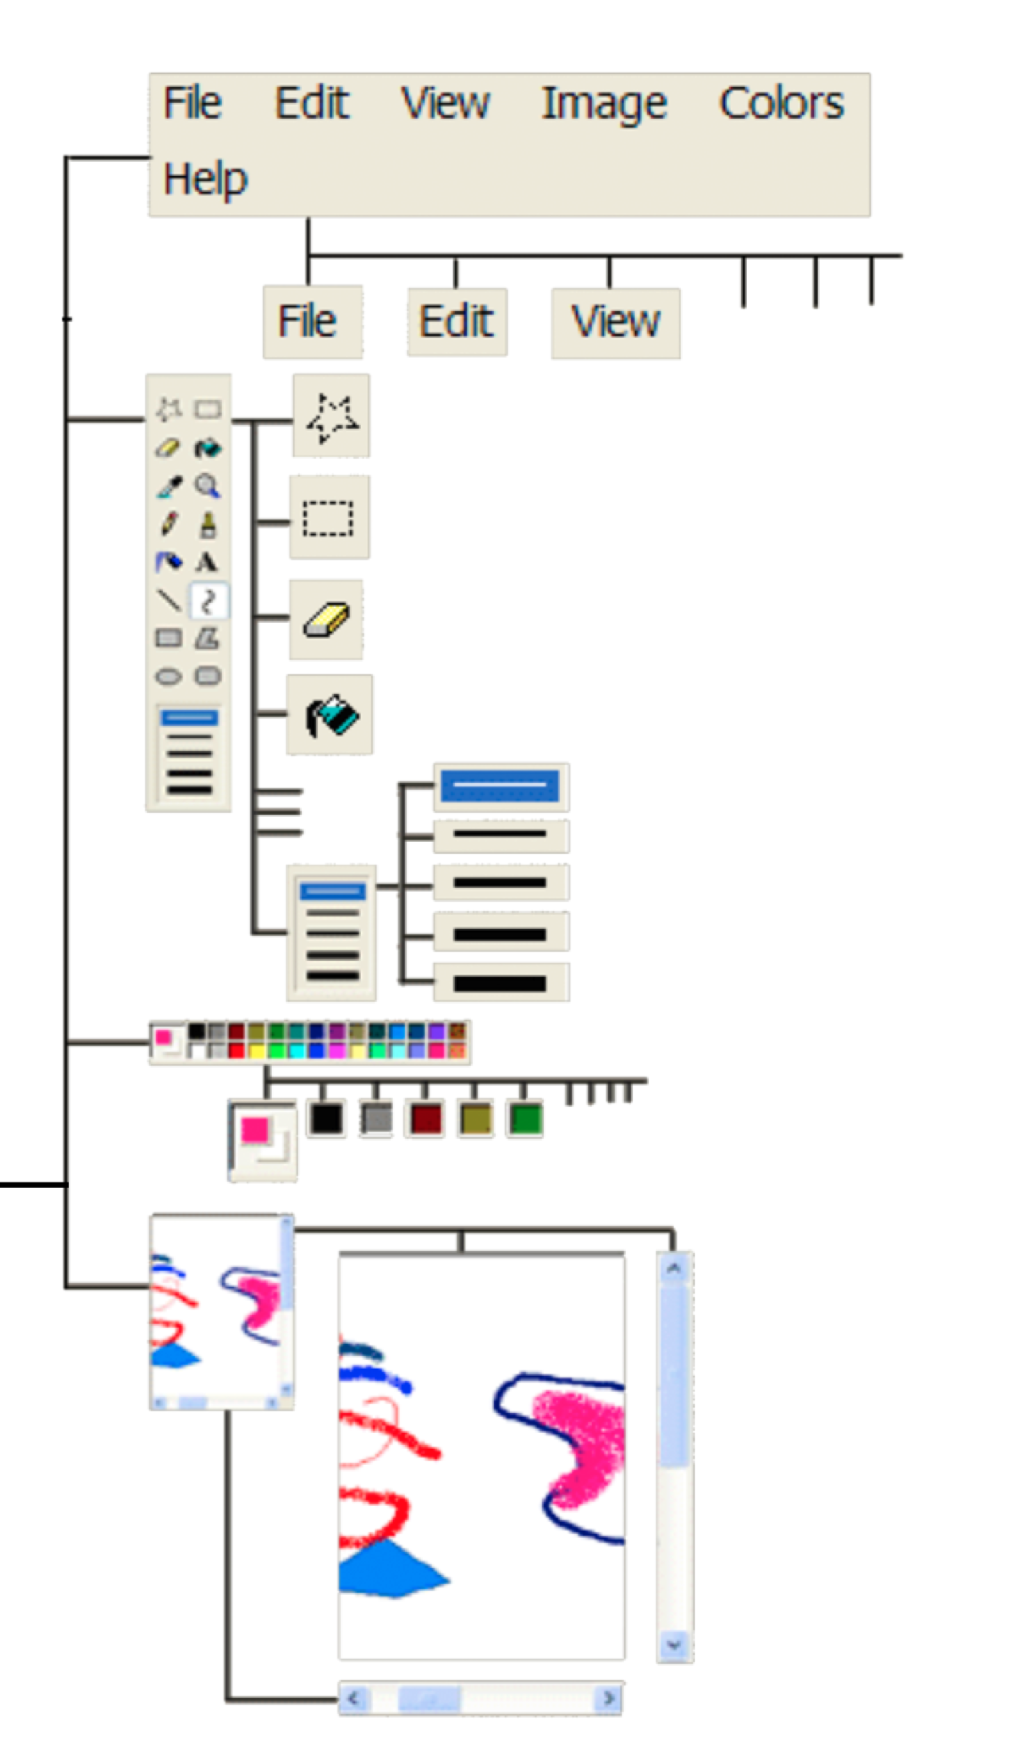
\includegraphics[scale=0.4]{25}
\end{center}

\subsection{Lightweight vs Heavyweight Widgets}
\begin{itemize}
\item Heavyweight widgets
\begin{itemize}
\item Widget toolkit wraps native-OS widgets
\item BWS/OS provides a hierarchical “windowing” system for all
widgets across all applications, and treats a widget essentially as a window
\item BWS can dispatch events to a specific widget
\item e.g. nested X Windows, Java’s AWT, HTML forms, Windows MFC
\end{itemize}
\item Lightweight widgets
\begin{itemize}
\item The widget toolkit draws its own widgets and is responsible for
mapping incoming events to widgets
\item BWS/OS dispatches to the window (NOT the widget) 
\item e.g. Java Swing, JQuery UI, Windows WPF
\end{itemize}
\end{itemize}


\end{document}





